\documentclass[12pt]{article}
\usepackage[margin = 1in]{geometry}

%<<<<<<< HEAD
% Load basic but necessary packages
\usepackage{amsmath, amsthm, amsfonts, setspace, mathrsfs}
\usepackage{enumerate}
\usepackage{enumitem}
\usepackage{graphicx, subfigure}
%\usepackage{chemfig}
%\usepackage{url, tikz}

%\usepackage{hyperref}
%	\hypersetup{colorlinks=true,
%				linkcolor=blue,
%				urlcolor=magenta,
%				citecolor=orange,
%				linkbordercolor=lightgray}
%	\urlstyle{same}

\usepackage{theoremref}
	
%=======

%\usepackage{amsmath, amsthm, setspace, theoremref, mathrsfs, enumerate, enumitem, amsfonts, url, tikz, chemfig}  

%>>>>>>> dc17b5dfcce777fa7b6515070cc8c1b8ac513e68

% Chemistry package - allows for notating chemical symbols and formulas
\usepackage[version=4]{mhchem}

% Glossary package - it is supposed to set up the symbols and abbreviations page(s) (not working yet [10 Apr 201])
%\usepackage[xindy,toc,ucmark,style=long3colheader,counter=equation]{glossaries}
%	\makeglossary

\usepackage[backend=bibtex,style=authoryear,maxcitenames=2, natbib=true, labelalpha=true]{biblatex} 	% Use the bibtex backend with the author year citation style (which resembles APA)
\addbibresource{PhD_Dissertation_Refs.bib}	% The file name of the bibliography
\addbibresource{optimizationBib.bib} 		% The file name of the bibliography

%%%% Glossary for Symbols and Abbreciations %%%%

% Redefine the way hyperref creates the target for equations
% So that the glossary links to equation numbers work
%\renewcommand*\theHequation{\theHchapter.\arabic{equation}}

% Change the glossary headings
%\renewcommand{\entryname}{Notation}
%\renewcommand{\descriptionname}{Function Name}
%\renewcommand{\pagelistname}{Number of Formula}

%\newglossaryentry{M}{name={\ensuremath{M}},
%					 sort=M,
%					 description={An index set of the sensors}}

%%%%  		End of Glossary Preamble 		%%%%

% Theorem Commands
\newtheorem{MyAssum}{}
\renewcommand{\theMyAssum}{\textbf{A\arabic{MyAssum}}}

\newtheorem*{conjecture}{Conjecture}

% Other Commands
\newcommand{\hcD}{\widehat{\mathcal{D}}}
\newcommand{\cD}{\mathcal{D}}
\newcommand{\deltaOTC}{\delta_{13}C}
\newcommand{\cM}{\mathcal{M}}
\newcommand{\cP}{\mathcal{P}}
\newcommand{\setbar}{\text{ }|\text{ }}

% Preamble
\begin{document}
	\section*{Preamble}
	This page is supposed to contain abbreviations, acronyms, and symbols with links to those in text.  Not currently working as of 08 Feb 2019.
	
	\par \noindent
	The following is a list of notation used in the model.
	\begin{enumerate}
		\item $F = [0, b_{1}] \times [0, b_{2}]$--The observation field.
		\item $f:\mathbb{R} \to \mathbb{R}$--The measurement certainty function based on distance to a measured site.
		\item $\cM$--An index set of the sensors.
		\item $P$--An index set of the discretized field.
		\item $G \subseteq F$--The gravel terrain (or other terrain) in which sensors cannot be placed.
		\item $r$--The minimum distance between sensors
		\item $\hcD: F \to \mathbb{R}$--The estimated isotope level at a site based on the measurements taken.
		\item $\cD: F \to \mathbb{R}$--The true isotope level at a site.
	\end{enumerate}
	
	\thispagestyle{empty}
	
	%\gls{M} 
	%\printglossary

% Start sections
	\newpage
	
	\section{Overview}
	\subsection{Introduction}
	The Earth remains a habitable planet largely in part to the greenhouse gases (GHG) such as methane (\ce{CH4}) and carbon dioxide (\ce{CO2}) that insulate the Earth by absorbing and emitting infrared radiation. Properly accounting for the pathways of GHGs into the atmosphere is essential to mitigating climate warming.
	
	\vspace{3mm}  \par \noindent
	Studies and long-term monitoring for changes in \ce{CO2} have been heavily documented for decades \citep{Keeling1960, Friedlingstein2014}. However, \ce{CH4}, is also an important GHG; one molecule of \ce{CH4} traps 86 times more thermal energy than a molecule of \ce{CO2} over a 20-year period and there are even claims that estimate is too low \citep{Howarth2015, Bridgham2013}. This ratio, also known as global warming potential has stimulated research during the last decade or so on the routes \ce{CH4} takes to enter the atmosphere. Though human-derived, or anthropogenic, sources are important to quantify, natural reservoirs of \ce{CH4} contribute about 51\% of total emissions in the previous decade \citep{Kirschke2013}. But estimates for natural sources currently contain a greater degree of uncertainty than their anthropogenic counterparts \citep{Kirschke2013}. 
	
	\vspace{3mm}  \par \noindent 
	Wetlands are the dominant source of natural production of \ce{CH4}, but they alone only account for about 60\% of natural emission, leaving the remaining 40\% to microbial activity in the soil microbes, termites, and even the deep ocean \citep{Kirschke2013, Etiope2002a}. Another important natural source of \ce{CH4} are derived from ongoing geologic processes, otherwise known as geogenic. Currently, geogenic emissions are estimated to produce 30-70 Mt \ce{CH4} yr$^{-1}$, which is on par with other non-wetland natural sources \citep{Etiope2002a}. This estimate was calculated by measuring \ce{CH4} from active points of emission (e.g. vents and fumaroles) and diffuse areas (thermally altered earth).
	
	
	\vspace{3mm}  \par \noindent 
	However, previous estimates are only from European locations, thus stimulating a need for diffuse \ce{CH4} measurements in N. America. This research seeks to further constrain estimates of \ce{CH4} emissions by providing the first geologic measurements of diffuse \ce{CH4} in N. American volcanic caldera and hydrothermal environments, specifically, Valles caldera (VC) and Yellowstone caldera (YC). Furthermore, collection of \ce{CH4} and \ce{CO2} emissions from numerous sites within VC and YC will permit the characterization of spatial and temporal variability; upon integrating that variability we will be able to: \textbf{estimate total emissions, assess correlations between emissions and/or geyser activity with time and space to constrain subsurface transport mechanisms, and lastly, make overall comparisons between the two calderas to highlight controls between emission rates}.
	
	\subsection{Site Description}
	A collapsed caldera is a large, basin-shaped depression formed by the collapse of the roof of a volcano following a large eruption. Valles Caldera is located in northcentral New Mexico and is one of several features within the Jemez Mountain Volcanic Field. VC initially erupted 1.2 million years ago, creating a caldera 20 km in diameter \citep{Goff2009}. Yellowstone Caldera is located in northwestern Wyoming and is a product of the North American plate moving west across a stationary mantle hotspot, causing linear chain of volcanic eruptions \citep{Smith1994}. An eruption 640 thousand years (kya) created YC and left behind a caldera that is roughly 64 km across. The most recent eruption at VC was 40 kya and for YC, 70 kya; these recent eruptions coupled with active hydrothermal systems reveal that both calderas are supplied with anonymously high subsurface heat sources. 
	
	\vspace{3mm}  \par \noindent	
	However, one important difference between the sites is that YC is more active than VC, which is exemplified with the greater abundance of thermal features, higher surface heat flow, and larger and more frequent earthquakes \citep{Lowenstern2008}. Together, VC and YC are two of the three major Quaternary calderas in the US and both are considered active volcanoes, making them relevant candidates for quantifying the contribution of geologic CH4 into the atmosphere.
	
	\subsection{Research Design \& Data Collection Methods}
	Emissions will be measured by capturing \ce{CH4} and \ce{CO2} as it migrates from the subsurface toward the atmosphere using a chamber sealed tightly to the surface. This Eosense autochamber (eosAC) will be connected to a Picarro G2201-i Cavity Ring-Down Spectrometer (CRDS) that can measure both gases rapidly (4 Hz) and in situ for concentrations ([\ce{CH4}] and [\ce{CO2}]) and carbon isotopic composition ($\delta^{13}$C-\ce{CH4} and $\delta^{13}$C-\ce{CO2}). Over several years, I have created a successful methodology that I will continue to use for these measurements. The concentration data will be necessary for making emission estimates and the carbon isotopic composition will be essential for characterizing the source of the gases and the temperature at which these gases formed. 
	
	\vspace{3mm}  \par \noindent 	
	Research shows the effectiveness of the CRDS-eosAC method \citep{Christiansen2015a}, but mobility is limited due to weight of the equipment ($> 54$ kg). For sites that I cannot access with the CRDS-eosAC method, I will use static PVC chambers \citep{Livingston2006}. Gas samples are withdrawn from the chamber headspace with a syringe and injected into a vial. \ce{CH4} concentration and $\delta^{13}$C-\ce{CH4}, and $\delta^{2}$H-\ce{CH4} will be shipped to UC Davis for GC-IRMS analysis. CO2 concentration and $\delta^{13}$C-\ce{CO2} will be measured using a GC-MS at the Center for Stable Isotopes (Univ. of New Mexico) with our collaborator, Prof. Tobias Fischer. 
	\section{Sensor Optimization Formulation}

\noindent
We formulate a nonlinear optimization algorithm to place sensors in the field in order to characterize the gaseous output in a given area. The model captures phenomena intrinsic to the "area" of the specific application and the "sensor" hardware. For instance, it is known that once a sensor's location has been chosen, the sensor can continuously record the concentration of carbon dioxide ([\ce{CO2}]), methane ([\ce{CH4}]), and carbon isotopes of methane ($\delta^{13}$\ce{C-CH4}), and carbon dioxide ($\delta^{13}$C-\ce{CO2}) measurements. Each of these measurements can be used to estimate, with relatively high precision \citep{Christiansen2015}, the isotopic composition at a specific location. That is, if $\hcD_{meas}$ is a function that represents the estimated \textbf{isotope} level after a complete set of measurements, and $\cD$ is a function that represents the true isotope level, then the difference between the two function values at a measured location is small. Hence, we make the following assumption:

\begin{MyAssum}\thlabel{exact}
Let $x$ be a chosen measurement site. Then $\cD(x) = \hcD(x)$.
\end{MyAssum}

\textit{We should be able to relax this assumption to say $||\cD(x) - \hcD(x)|| < \epsilon$.}\\


\begin{subequations}\label{PreliminaryModel}
\begin{align}                                               
\min \ &\sum\limits_{p \in P}\sum\limits_{m \in \cM} \frac{f(x)}{|\cM|} \\
\text{s.t.} & x_{m} \in F \backslash G, \forall \ m \in \cM, \label{PM:gravelConstraint}\\
&x \in \cP, \forall \ m, m' \in \cM, m \neq m'. \label{PM:radiusConstraint}
\end{align}
\end{subequations}
General constraints are represented by $x \in \cP$.

There are multiple choices of objectives functions one can use to model the decay in a measurement value as a function of the distance to the specified site. For ease of exposition, we introduce variables $y_{p,m} = x_{m} - X_{p}$, where $x_{m}$ is the location of a sensor and $X_{P}$ is a desired measurement site. Note that this produces an affine constraint in the formulation. 

Consider $f_{1}: \mathbb{R}^{2} \to \mathbb{R}$ defined by $f_{1}(z) = ||z||_{2}^{2}$. Then $f_{1}$ is a convex function. Define $F_{1}: \mathbb{R}^{2\times |\cM|} \times \mathbb{R}^{2 \times |\cM| \times |P|}$ by $F_{1}(x,y) = \sum\limits_{p \in P}\sum\limits_{m \in \cM} \frac{1}{\cM}f_{1}(y_{p,m})$. Then $F_{1}$ is a convex objective function. A similar result occurs if $f_{2}:\mathbb{R}^{2} \to \mathbb{R}$ is defined by $f_{2}(z) = e^{||z||_{2}^{2}}$ and $F_{2}: \mathbb{R}^{2\times |\cM|} \times \mathbb{R}^{2 \times |M| \times |P|}$ is defined by $F_{2}(x,y) = \sum\limits_{p \in P}\sum\limits_{m \in M} \frac{1}{M}f_{2}(y_{p,m})$. 

A common objective function is the \textit{Gaussian}. Let $f_{3}: \mathbb{R}^{2} \to \mathbb{R}$ be defined by $f_{3}(z) = e^{-\frac{||z||^{2}_{2}}{\sigma}}$, where $\sigma > 0$ is a parameter. The Gaussian function $f_{3}$ is a log-concave function; hence, it is a quasiconcave function. Let $F_{3}:\mathbb{R}^{2\times |M|} \times \mathbb{R}^{2 \times |M| \times |P|}$ be defined by $F_{3}(x,y) = \prod\limits_{p \in P}\prod\limits_{m \in M} \frac{1}{M}f_{3}(y_{p,m})$. Then, $F_{3}$ is the product of log-concave functions and is log-concave. Moreover, $-F_{3}$ is quasiconvex.


\subsection{A Connection to K-means}
Formulation \eqref{PreliminaryModel} can be adapted slightly into a special case of K-means. To do so, we introduce binary variables and ``big-M" constraints that model which sensor is closest to each location. In addition, we first assume that $G = \emptyset$ and that $F$ is a convex set. 

\begin{subequations}\label{KMeansModel}
	\begin{align}                                               
	\min \ \sum\limits_{p \in P}\sum\limits_{m \in \cM} &\frac{y_{p,m}}{|\cM|} \\
	\text{s.t.}\  & x_{m} \in F \forall \ m \in \cM, \\
	&y_{p,m} \geq ||x_{m} - X_{p}||_{2}^{2} - M(1 - z_{p,m}),\\
	\sum\limits_{m \in \cM} &z_{p,m} = 1,\\
	&y_{p,m} \geq 0, \forall \ m \in \cM, p \in P,\\
	&z_{p,m} \in \mathbb{B}, \forall \ m \in \cM, p \in P.
	\end{align}
\end{subequations}

\begin{conjecture}\thlabel{KMeansConjecture}
There exists an optimal solution ($x^{*}, y^{*}, z^{*}$) to \eqref{KMeansModel} such that $x^{*}_{m}$ is the mean of $\{X_{p}\}_{P(m)}$, where $P(m) = \{p \in P : z_{p,m} = 1\}$.\footnote{Maybe we can also show that it is the unique optimal solution. Or analyze that case.}
\end{conjecture}

In general, $G \neq \emptyset$. Hence, it is possible that the the K-means solution is infeasible. This leads to a \textit{constrained K-means} model. There are examples of constrained K-means models in the literature. For instance, \citep{Wagstaff2001} considers constraints that either ensure two instances are assigned to the same cluster or  prevent two instances from sharing a cluster. \citep{Luo2003} considers a spatially constrained K-means algorithm with applications to image segmentation. Spatial constraints are useful in image segmentation because they require that the clusters are contiguous; in an image, the pixels in each cluster form a connected subset.

To the best of our knowledge,\footnote{Need to increase our knowledge here...} this is the first study of what we call \textit{terrain constrained} K-means: the centroids are constrained away from subsets of the feature space.

In addition, we also propose using alternative distance metrics from the Euclidean norm, as proposed by \citep{Aggarwal2001}.

\subsection{Reverse Convex Programming}
Due to the constraint \eqref{PM:gravelConstraint}, this optimization will probably be at best a Reverse Convex Program \citep{Hillestad1980}. Further reading to be done at \url{https://link.springer.com/content/pdf/10.1007/BF01442883.pdf}. \cite{Hillestad1980} describe how to identify basic solutions and they also provide a cutting plane algorithm.

If one assumes that the untestable areas $\mathcal{G}$ in the interior of the cite can be modeled by circles, then this can be modeled by $g_{k}(x) = ||x - c^{k}||_{2}^{2} - d^{k} \geq 0$, where $c_{k}$ is the center of the restricted area. Because $g_{k}$ is strictly convex, $g_{k}$ is also strictly quasiconvex. Moreover, $g_{k}$ is continuous so the constraint is a reverse convex constraint. Other restrictions are also possible. For example, an ellipsoidal constraint can be modeled as $g_{k}(x) = ||x - c^{k}||_{E_{k}}^{2} - d^{k} \geq 0$, where $E_{k}$ is a diagonal matrix in $\mathbb{R}^{2}_{++}$ in which its nonzero entries dictate the lengths of the semi-axes. Polyhedral restrictions are not given by reverse convex constraints; however, one can approximate them using strictly convex functions. For instance, given the reverse $L_{1}$-norm constraint $||x - c^{k}||_{1} - d^{k} \geq 0$, one can approximate this constraint by $g_{k}(x) = ||x - c^{k}||_{p}^{p} - (d^{k})^{p} \geq 0$, for some $p > 1$.

Suppose that the restricted area $\mathcal{G}$ is given by multiple ellipsoids centered around point $c_{k}, k = 1,...,K$. Given that $x_{m}$ represents the placement of sensor $m \in \{1,...,M\}$ in the 2-dimensional space, the restricted area can be modeled by multiple reverse convex constraints with convex functions $g_{m,k}: \mathbb{R}^{2M} \to \mathbb{R}$ defined by $g_{m,k}(x) = ||x_{m} - c_{k}||^{2}_{E_{k}} - d_{k}$, where $E_{k} \in \mathbb{R}^{2}_{++}$ is the diagonal matrix defining the ellipsoid semi-axes and $d_{k} \geq 0$. 
Then, $\mathcal{G} = \{x \in \mathbb{R}^{2M} \setbar g_{m,k}(x) < 0, \text{for some } m \in \{1,...,M\}, k \in \{1,...,K\}\}$.

The optimization problem now has multiple reverse convex constraints:
\begin{subequations}\label{multipleReverseModel}
\begin{align}                                               
\min \ &\sum\limits_{p \in P}\sum\limits_{m \in \cM} \frac{f(x)}{|\cM|} \\
\text{s.t.} & x_{m} \in F, \forall \ m \in \cM, \label{mR:gravelConstraint}\\
& g_{m,k}(x) \geq 0, \forall \ m \in \{1,...,M\}, k \in \{1,...,K\}, \\
&x \in \cP, \forall \ m, m' \in \cM, m \neq m'. \label{mR:radiusConstraint}
\end{align}
\end{subequations}

Many reverse convex algorithms are designed for only a single reverse convex constraint (see Tuy other works to cite). It is shown in (Jacobsen Encyclopedia entry) that one can transform a problem with multiple reverse convex constraints into one with a single reverse convex constraint, and we provide details specific to this setting.

Let $s, p_{m,k}, q: \mathbb{R}^{2M} \to \mathbb{R}$, for all $k \in \{1,...,K\}, m \in \{1,...,M\}$, where $s(x) = \sum\limits_{k = 1}^{K}\sum\limits_{m = 1}^{M} g_{m,k}(x)$, $p_{m,k}(x) = s(x) - g_{m,k}(x)$, and $q(x) = \max\limits_{k \in \{1,...,K\}, m \in \{1,...,M\}} p_{m,k}(x)$. Then constraint \eqref{mR:gravelConstraint} is equivalent to the following two constraints with the auxiliary variable $t \in \mathbb{R}$:
\begin{align*}
& q(x) - t \leq 0,\\
& s(x) - t \geq 0,
\end{align*}
where the first constraint is a convex constraint and the second constraint is a reverse convex constraint. Thus, if \eqref{multipleReverseModel} is a convex program with multiple additional reverse convex constraints, then \eqref{multipleReverseTransformedModel} is a convex program with a single reverse convex constraint.

\begin{subequations}\label{multipleReverseTransformedModel}
\begin{align}                                               
\min \ &\sum\limits_{p \in P}\sum\limits_{m \in \cM} \frac{f(x)}{|\cM|} \\
\text{s.t.} & x_{m} \in F, \forall \ m \in \cM, \label{mRT:gravelConstraint}\\
& s(x) - t \leq 0,\\
& q(x) - t \geq 0,\\
&x \in \cP, \forall \ m, m' \in \cM, m \neq m'. \label{mRT:radiusConstraint}
\end{align}
\end{subequations}


Returning to the K-means structure, the $z$ variables indicate whether a sensor is assigned to a location. These variables are binary, but these binary constraints can be expressed with reverse convexity:

\begin{align*}
&\{z \in \mathbb{B}^{MK}\} = \{z \in \mathbb{R}^{MK}_{+} \setbar h(z) \geq 0\},\\
&h(z) = \sum\limits_{m = 1}^{M}\sum\limits_{k = 1}^{K} z_{mk}(z_{mk} - 1).
\end{align*}

Thus, one can adapt $s$ and $q$ to include $h$ as one of the functions along with $g_{mk}$ to create a reverse convex program without integrality constraints.
	\section{Monte Carlo Simulation of Synthetic Data}

% Discussion of how observed points were measured and located
\noindent
Before beginning with the implementation of the Monte Carlo simulation, it is pertinent to explain the sampling procedure as  it took place in the field.  These points will be referred to as the \textit{observed} points henceforth.  From site to site, 4-10 observed points were measured each day, with some sites having more than 4-10 observed points when measurements were repeated (e.g. GVNT).  

% Defining sample spaces and distribution of observed points
\vspace{3mm} \par \noindent
For this study, sample spaces are defined by ways: 1) by name and 2) geographically.  A sitename (e.g. EETR, GVNT, MMTH) defines the name of a sample space. Geographically, sample spaces were defined from images drawn from Google Earth Pro. After the observed points were uploaded to Google Earth Pro, an image capturing the points and the surrounding area (30-50 meters in each direction from the center of of observed points) was downloaded and used as the sample space.  Figure 1 highlight an example of the sample space at PRCN is defined geographically.

\begin{figure}[h]
    \centering
    \subfigure[]
    {
        \label{fig:first}
        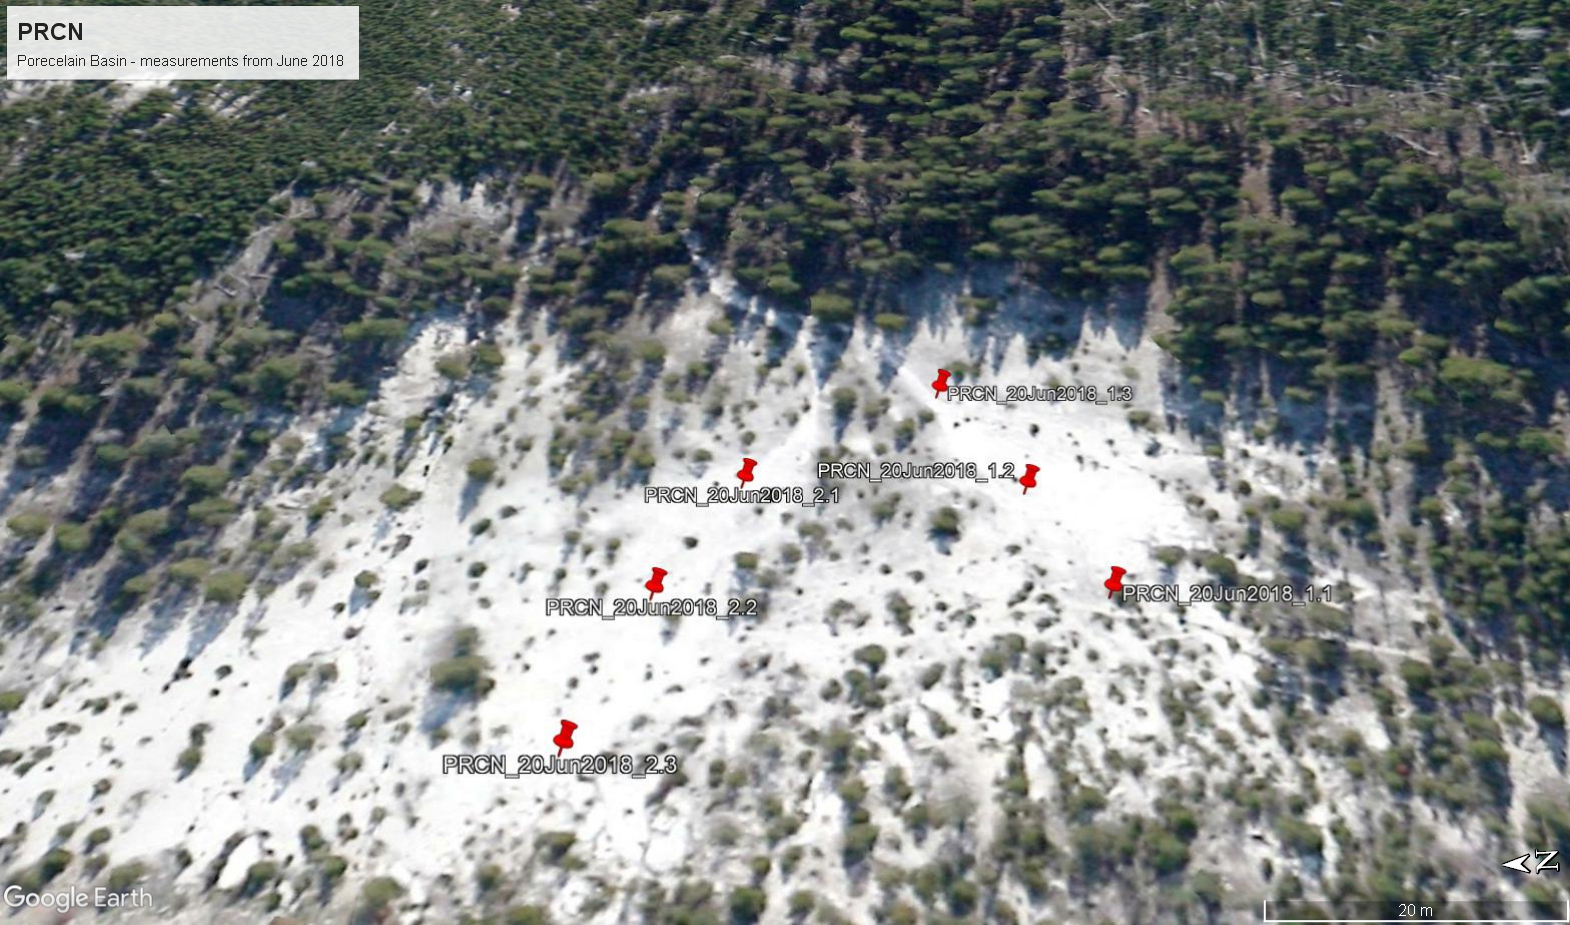
\includegraphics[width=0.6\textwidth]{Figures/PRCN_2018_Sampling_Locations.jpg}
    }
    \subfigure[]
    {
        \label{fig:second}
        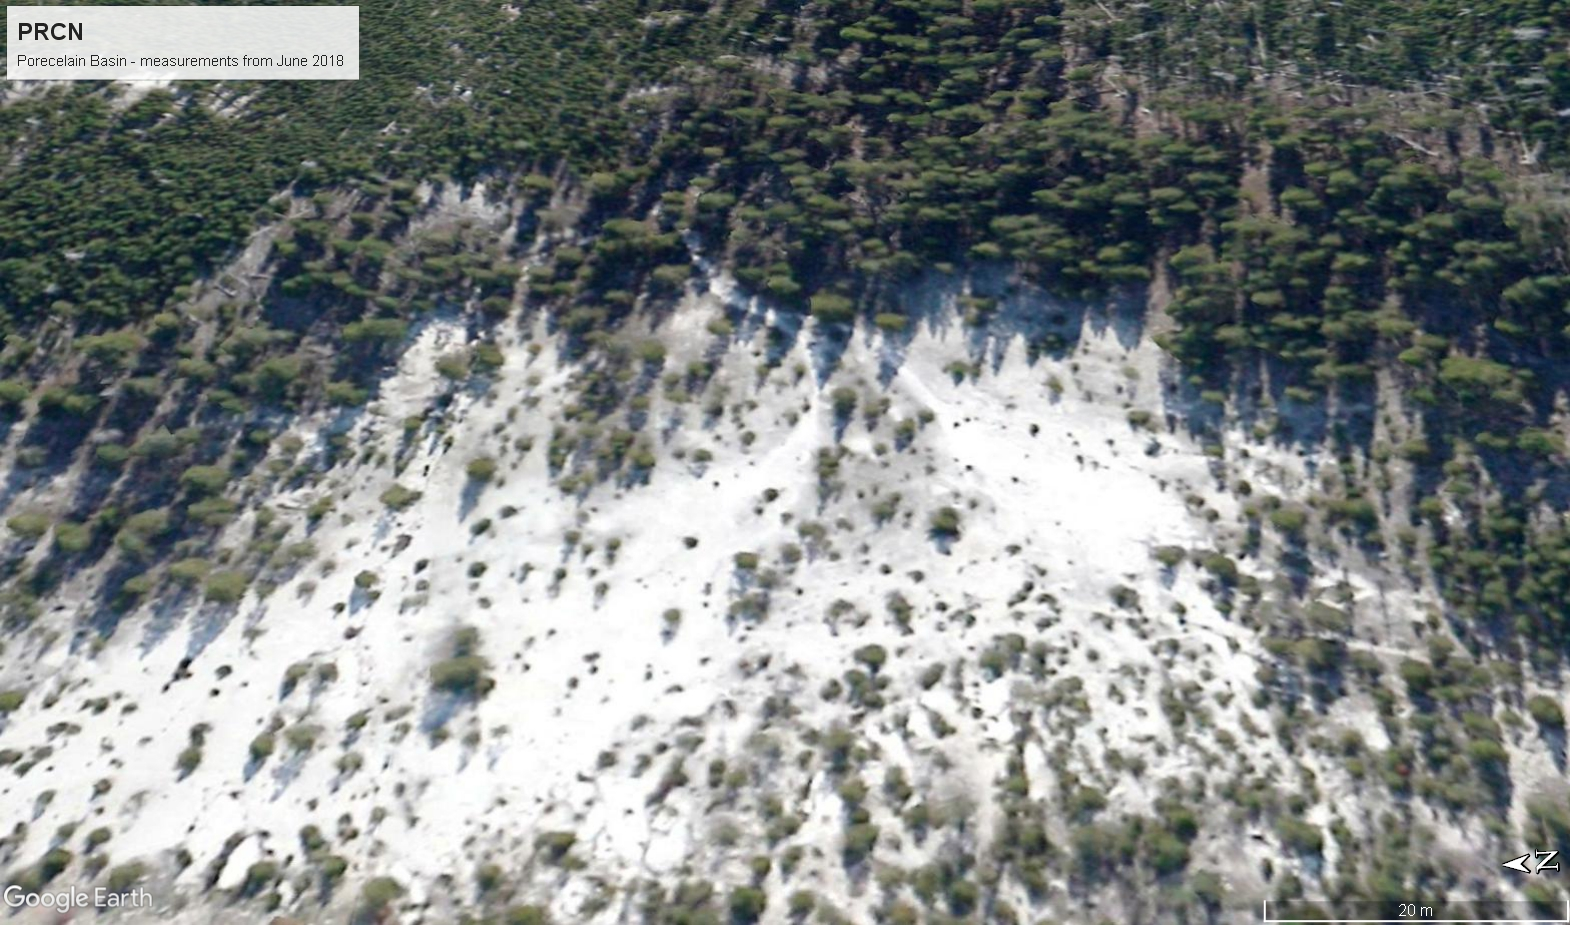
\includegraphics[width=0.6\textwidth]{Figures/PRCN_2018_Sampling_Locations_no_LABELS.jpg}
    }
    \caption{Sampling spaces at PRCN, shown with (a) and without (b) the location of the observed points}
    \label{fig:subfigures}
\end{figure}

% Distribution of observed points
\vspace{3mm} \par \noindent
With the sample space defined, the distribution of observed points was analyzed to assess if they were
	\section{Some Implementation Notes}
The workflow for solving the problem looks like:
\begin{enumerate}
\item Read in image of the field site
\item Using colors determine which areas are off limits
\item Use ellipses to cover the off-limit areas for the reverse convex model
\item Solve the sensor placement problem 
\item Using some simulation, determine the collected ``data" by the algorithmically placed sensors
\item Create model for entire field
\item Compare to simulated truth
\end{enumerate}


% Bibliography
\newpage
\printbibliography[heading=bibintoc]

\end{document}